\chapter{Methodologie}
\label{hoofdstuk:3}

We zullen zowel bij het vergelijken van de uiteindelijke algoritmes in hoofdstuk \ref{hoofdstuk:resultaten} als bij het vergelijken van verschillende technieken en parameterwaarden in hoofdstuk \ref{hoofdstuk:tucker} en hoofdstuk \ref{hoofdstuk:tensor_trains} experimenten uitvoeren om onze conclusies te staven. Om deze reden zullen we eerst alle nodige context voor deze experimenten beschrijven in dit hoofdstuk.

\section{Algemeen}
Om rekening te houden met variantie, zullen tijdsmetingen in deze tekst uitgemiddeld worden over 10 experimenten, tenzij anders vermeld. Technisch gezien zijn de resultaten van stochastische algoritmen ook niet compleet deterministisch, maar aangezien de variantie hierop vaak minimaal is zal de nood aan een grotere steekproef geval per geval behandeld worden. Daarnaast zullen tijdsmetingen ook uitgedrukt worden in CPU-tijd.

\section{Hardware}
Tenzij anders vermeld werden de tijdsmetingen in deze tekst uitgevoerd op \'e\'en core van een Intel(R) Core(TM) i7-4700HQ CPU @ 2.40GHz processor met 6GB RAM (waarvan meestal slechts een klein deel gebruikt werd weliswaar).

\section{Compressiefactor}

De compressiefactor is een belangrijke variabele die we zullen gebruiken in deze tekst. Hiermee hebben we het over de verhouding tussen de grootte van de originele, ongecomprimeerde 3D-tensor (dus bijvoorbeeld voor een $100 \times 100 \times 10$ tensor bestaande uit 16-bit integers is dit 200000 bytes) en de grootte van de gecomprimeerde versie. Dit is echter een erg simpel formaat en niet altijd de beste manier om deze data op te slaan. Men moet er dus rekening mee houden dat men zelfs door alleen simpele lossless compressie hierop uit te voeren al een compressiefactor van bv. 1.5 kan bekomen. Bijgevolg dient deze factor vooral relatief bekeken te worden, om verschillende compressietechnieken met elkaar te kunnen vergelijken.\\

Verder zal het geheugengebruik van metadata (afmetingen van tensoren, compressieparameters, ...) verwaarloosd worden, aangezien dit veel kleiner is dan de benodigde opslagruimte voor tensoren, matrices, ...

\section{Compressiefout}

Om de fouten ge\"introduceerd door de lossy compressie te vergelijken, zullen we werken met de relatieve fout, gedefinieerd als:

\[
\text{relatieve fout} = \frac{||\text{gereconstrueerde tensor} - \text{originele tensor}||_F}{||\text{originele tensor}||_F}
\]

\section{Implementatie}

De implementatie van de besproken algoritmen gebeurde in Python, waarbij het zware rekenwerk wordt uitgevoerd via library calls, voornamelijk aan de hand van NumPy/SciPy maar ook bijvoorbeeld zlib, ... Hierbij zijn ook alternatieve strategie\"en getest (zoals het al dan niet minimaliseren van transposities, het gebruik van \texttt{numpy.einsum}, ...), waarbij telkens de meest performante werd gekozen. Deze keuzes zullen niet behandeld worden in deze tekst vanwege de sterke afhankelijkheid van de gekozen programmeertaal. Desalniettemin kan het dat er nog steeds merkbare ineffici\"enties in de implementatie zijn.

\newpage
\section{Datasets}

Om een idee te krijgen van de effici\"entie van de verschillende compressietechnieken, moet men gebruik maken van echte hyperspectrale afbeeldingen. Hieronder volgen enkele voorbeelden met hun bijbehorende eigenschappen. De afbeeldingen zijn slechts een 2D-voorstelling van de volledige data, verkregen door alle frequentiekanalen bij elkaar op te tellen en deze sommen voor te stellen met grijswaarden.

\subsection{Cuprite}

\begin{figure}[H]
  \centering
  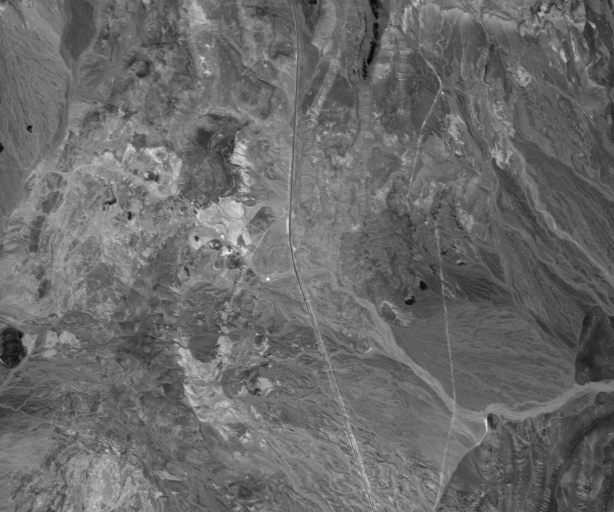
\includegraphics[scale=0.5]{images/cuprite_sum.png}
  \caption{Cuprite, VS. Bron: AVIRIS \cite{ref:cuprite}}.
  \label{fig:cuprite_sum}
\end{figure}

\textbf{Spatiale dimensies:} $512 \times 614$\\
\textbf{Spectrale dimensie:} 224 origineel, maar voor verder gebruik zijn de frequentiekanalen 0-3, 106-113, 152-168 en 219-223 verwijderd aangezien deze artefacten bevatten (banden met waarde 0, banden met veel te hoge, willekeurig verdeelde intensiteiten en naburige banden), dus de uiteindelijke spectrale dimensie is 190.

\subsection{Pavia Centre}

\begin{figure}[H]
  \centering
  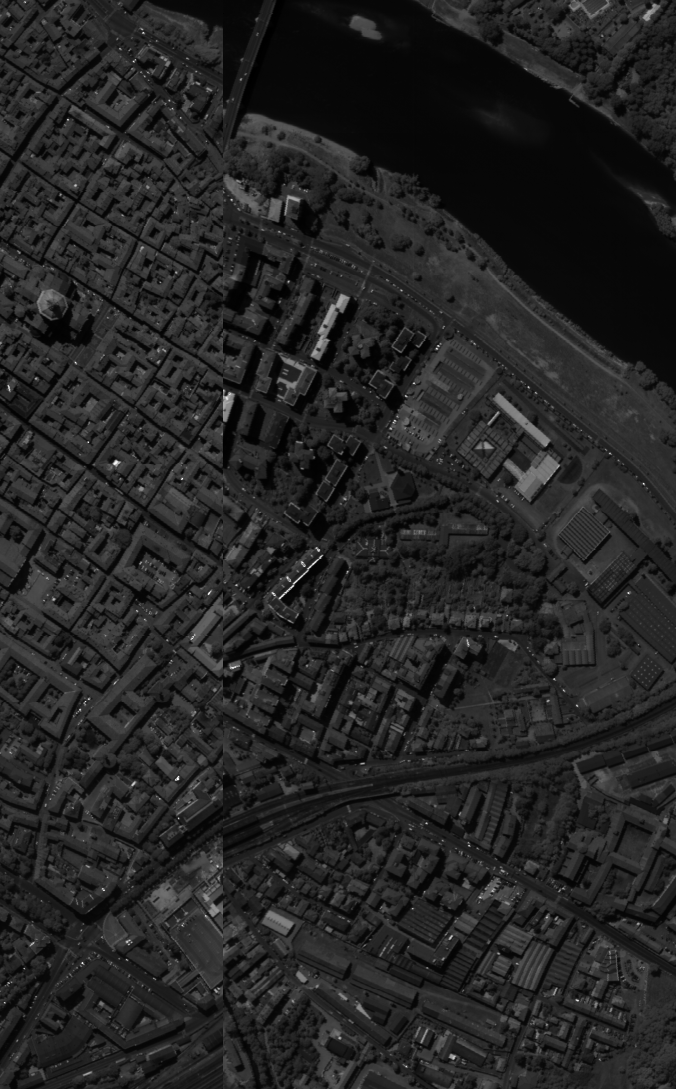
\includegraphics[scale=0.4]{images/pavia_sum.png}
  \caption{Pavia Centre, Itali\"e. Bron: ROSIS \cite{ref:pavia}}.
  \label{fig:pavia_sum}
\end{figure}

\textbf{Spatiale dimensies:} Na het verwijderen van de banden zonder informatie, $1096 \times 715$ (zie de download van \cite{ref:pavia}), maar om makkelijker te kunnen reshapen zullen we werken met de $1089 \times 676$ pixels met laagste indices.\\
\textbf{Spectrale dimensie:} 102